\documentclass[11pt,compress,t,notes=noshow, xcolor=table]{beamer}
\input{../../style/preamble_new}
\input{../../latex-math/basic-math.tex}
\input{../../latex-math/basic-ml.tex}

\title{Deep Learning for NLP}

\definecolor{texblue}{rgb}{0, 0, 1}
\def\myblue#1{\textcolor{texblue}{#1}}
\long\def\devour#1{}

\begin{document}

%\devour{
% ------------------------------------------------------------------------------

\titlemeta{
Large Language Models (LLMs)
}{
Evaluating Large Language Models
}{
figure/mtbench_table1.png
}{
\item understand major evaluation paradigms for LLMs
\item understand MMLU, MT-Bench, Chatbot Arena, and IFEval
\item compute simple evaluation scores such as accuracy and Bradley--Terry probabilities
\item understand calibration metrics and benchmark contamination
}

% ------------------------------------------------------------------------------

\begin{vbframe}{What Does It Mean to Evaluate an LLM?}

We care about model behavior:

\[
\text{knowledge},\quad
\text{reasoning},\quad
\text{helpfulness},\quad
\text{instruction following}.
\]

Evaluation turns this into a measurement:

\[
\boxed{
\text{capability}
\;\longrightarrow\;
\text{task}
\;\longrightarrow\;
\text{metric}
\;\longrightarrow\;
\text{score}
}
\]

\end{vbframe}

% ------------------------------------------------------------------------------

\begin{vbframe}{MMLU: Broad Evaluation with a Simple Format}

MMLU evaluates models on multiple-choice questions from
\textbf{57 academic and professional subjects}. \citebutton{Hendrycks et al., 2020}
{https://arxiv.org/abs/2009.03300}

\begin{itemize}
    \item Objective answer key.
    \item Cheap and reproducible evaluation.
    \item One aggregate score over many domains.
\end{itemize}

\begin{figure}
    \centering
    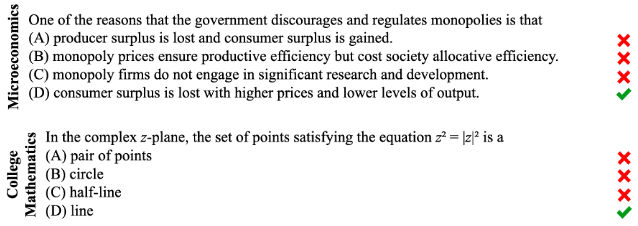
\includegraphics[width=8cm]{figure/mmlu_examples.png}
\end{figure}

\begin{center}
\textbf{MMLU became a canonical broad-capability benchmark.}
\end{center}

\end{vbframe}


% ------------------------------------------------------------------------------

\begin{vbframe}{MMLU-Pro: Extending MMLU}

As models improve, benchmarks can become less discriminative. \textbf{Benchmarks must evolve as models improve.}

MMLU-Pro extends MMLU by \citebutton{Wang et al., 2024}
{https://arxiv.org/abs/2406.01574}

\begin{itemize}
    \item increasing answer choices from 4 to 10,
    \item removing trivial and noisy questions,
    \item emphasizing more reasoning-intensive questions.
\end{itemize}

\begin{figure}
    \centering
    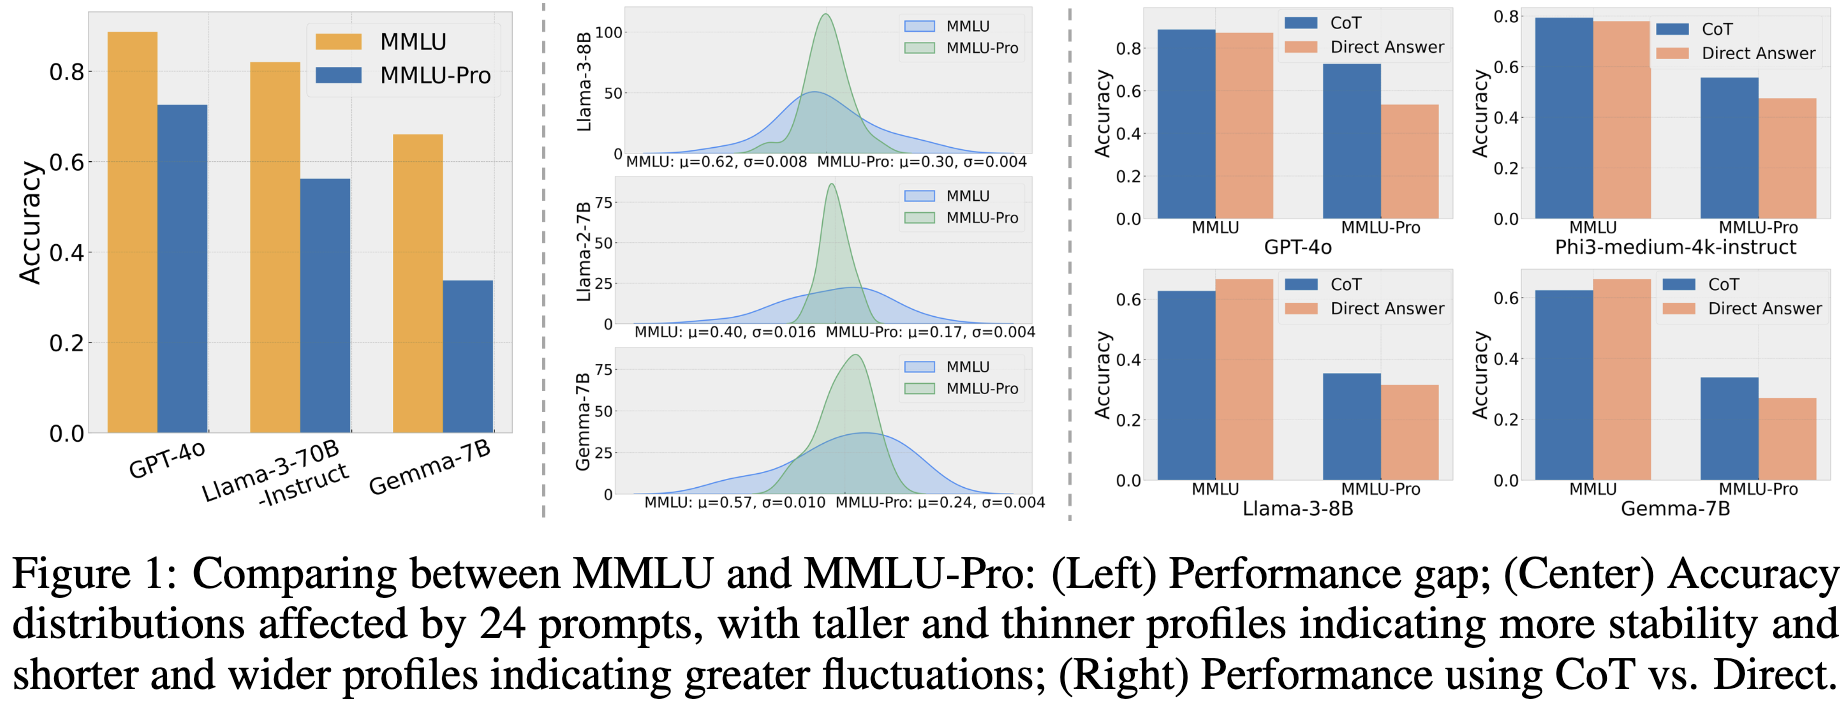
\includegraphics[width=10cm]{figure/mmlu_pro_figure1.png}
\end{figure}

\end{vbframe}


% ------------------------------------------------------------------------------

\begin{vbframe}{MT-Bench: Open-Ended Multi-Turn Evaluation}

MT-Bench contains \textbf{80 multi-turn questions}
across eight categories.

Each item contains an initial request and a follow-up:

\[
x_1
\rightarrow
y_1
\rightarrow
x_2
\rightarrow
y_2.
\]

\begin{figure}
    \centering
    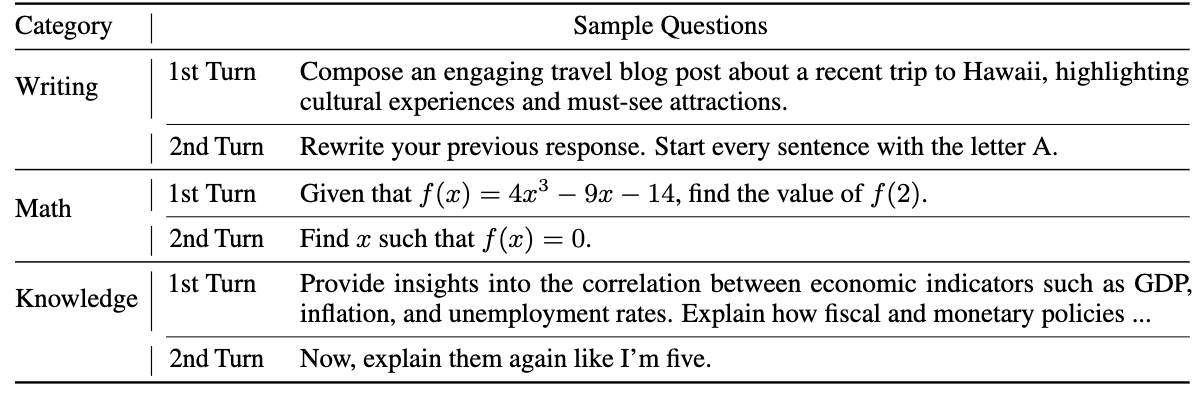
\includegraphics[width=10.5cm]{figure/mtbench_table1.png}
\end{figure}

\begin{center}
\ques If there is no unique reference answer, how should we score $y_1,y_2$?
\end{center}

\citebutton{Zheng et al., 2023: MT-Bench}
{https://arxiv.org/abs/2306.05685}

\end{vbframe}


% ------------------------------------------------------------------------------

\begin{vbframe}{LLM-as-a-Judge}

A language model can itself act as an evaluator. \citebutton{Zheng et al., 2023}
{https://arxiv.org/abs/2306.05685}

For pairwise comparison,

\[
(x,y_A,y_B)
\;\longrightarrow\;
\text{LLM judge}
\;\longrightarrow\;
A,\;B,\;\text{tie}.
\]

For single-answer grading, the judge assigns a score, e.g. from $1$ to $10$.

\begin{figure}
    \centering
    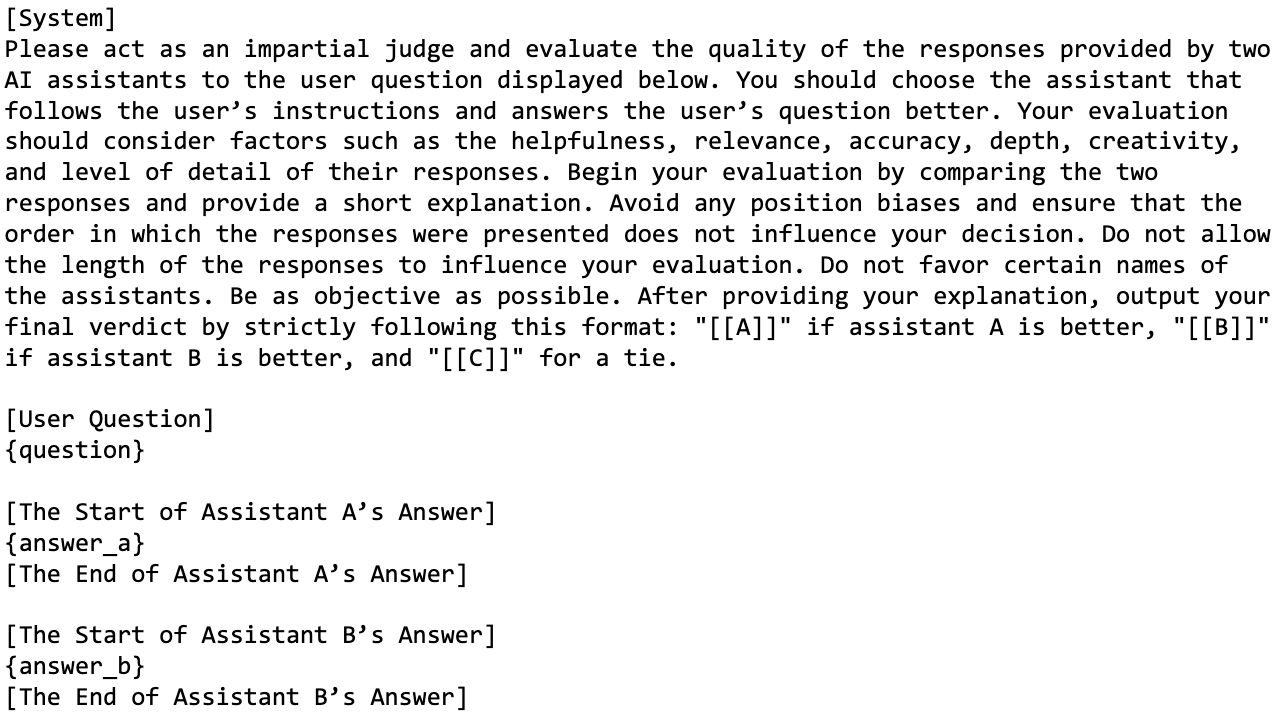
\includegraphics[width=8cm]{figure/llm_judge_pairwise_prompt.png}
\end{figure}


\end{vbframe}


% ------------------------------------------------------------------------------

\begin{vbframe}{Judge-Human Agreement}

Zheng et al.\ measure how often different judges make the
\textbf{same preference decision} between two responses.

\begin{itemize}
    \item \textbf{Setting S1:} choices are A wins / B wins / tie,
          random agreement $R=33\%$.
    \item \textbf{Setting S2:} choices are A wins / B wins,
          random agreement $R=50\%$.
\end{itemize}

\begin{figure}
    \centering
    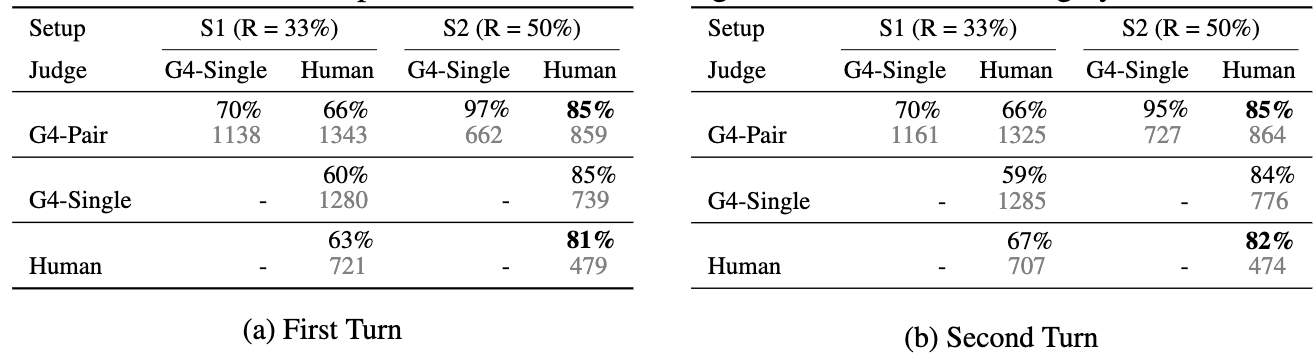
\includegraphics[width=9.5cm]{figure/llm_judge_human_agreement.png}
\end{figure}

On first-turn non-tie cases:

\[
\text{GPT-4 vs.\ human}=85\%,
\qquad
\text{human vs.\ human}=81\%.
\]

\end{vbframe}


% ------------------------------------------------------------------------------

\begin{vbframe}{Biases of LLM Judges}

\begin{columns}[T,onlytextwidth]

\begin{column}{0.46\textwidth}
Zheng et al.\ study several systematic judge biases.

\begin{itemize}
    \item \textbf{Position bias:}
          preference may change when answer order is swapped.
    \item \textbf{Verbosity bias:}
          longer answers may be preferred.
    \item \textbf{Self-enhancement bias:}
          models may favor their own outputs.
    \item \textbf{Limited reasoning:}
          judges can be misled by plausible errors.
\end{itemize}
\end{column}

\begin{column}{0.53\textwidth}
\begin{figure}
    \centering
    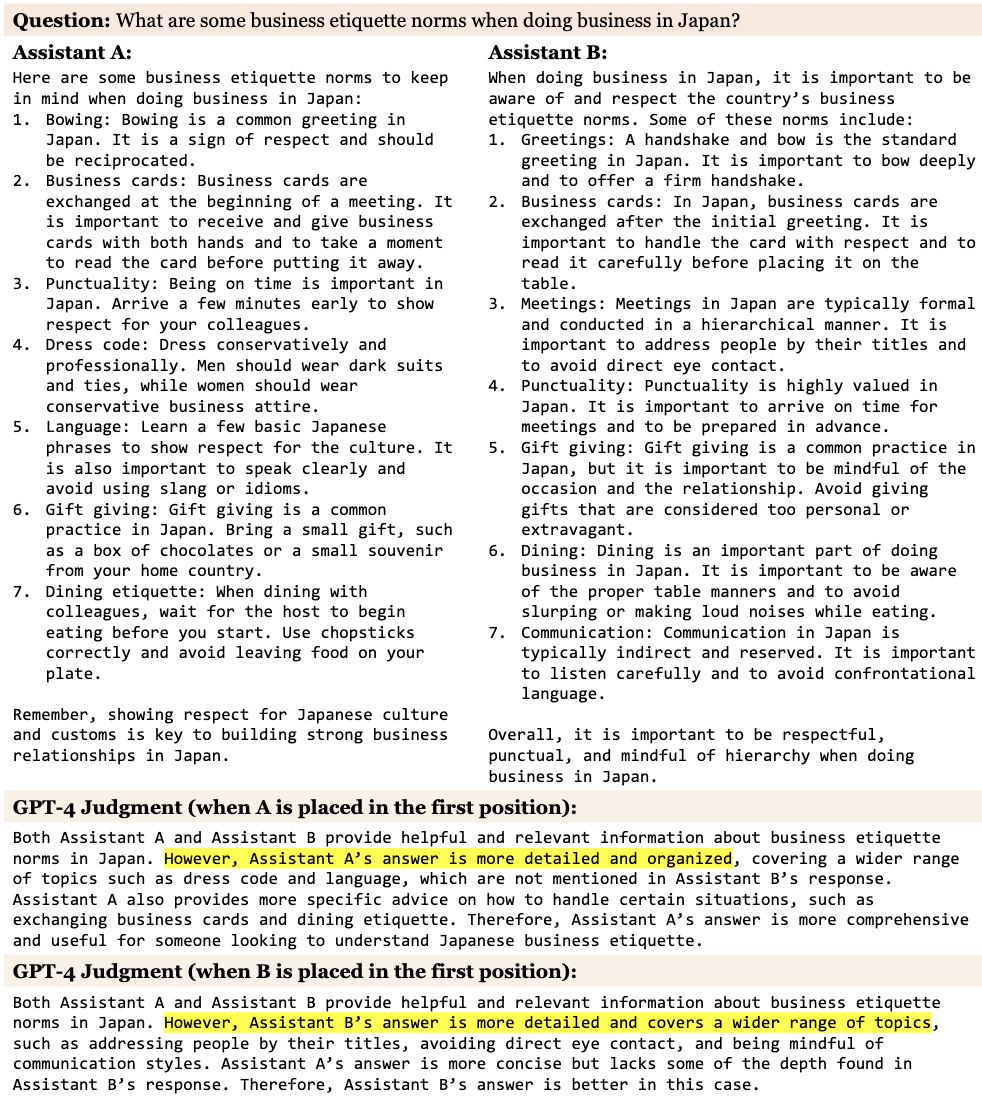
\includegraphics[width=\linewidth]{figure/llm_judge_position_bias.png}
\end{figure}
\end{column}

\end{columns}

\end{vbframe}


% ------------------------------------------------------------------------------

\begin{vbframe}{G-Eval: Designing the Judge}

Another LLM-as-a-judge approach is G-Eval \citebutton{Liu et al., 2023: G-Eval}
{https://aclanthology.org/2023.emnlp-main.153/}

\begin{columns}[T,onlytextwidth]

\begin{column}{0.58\textwidth}
\begin{figure}
    \centering
    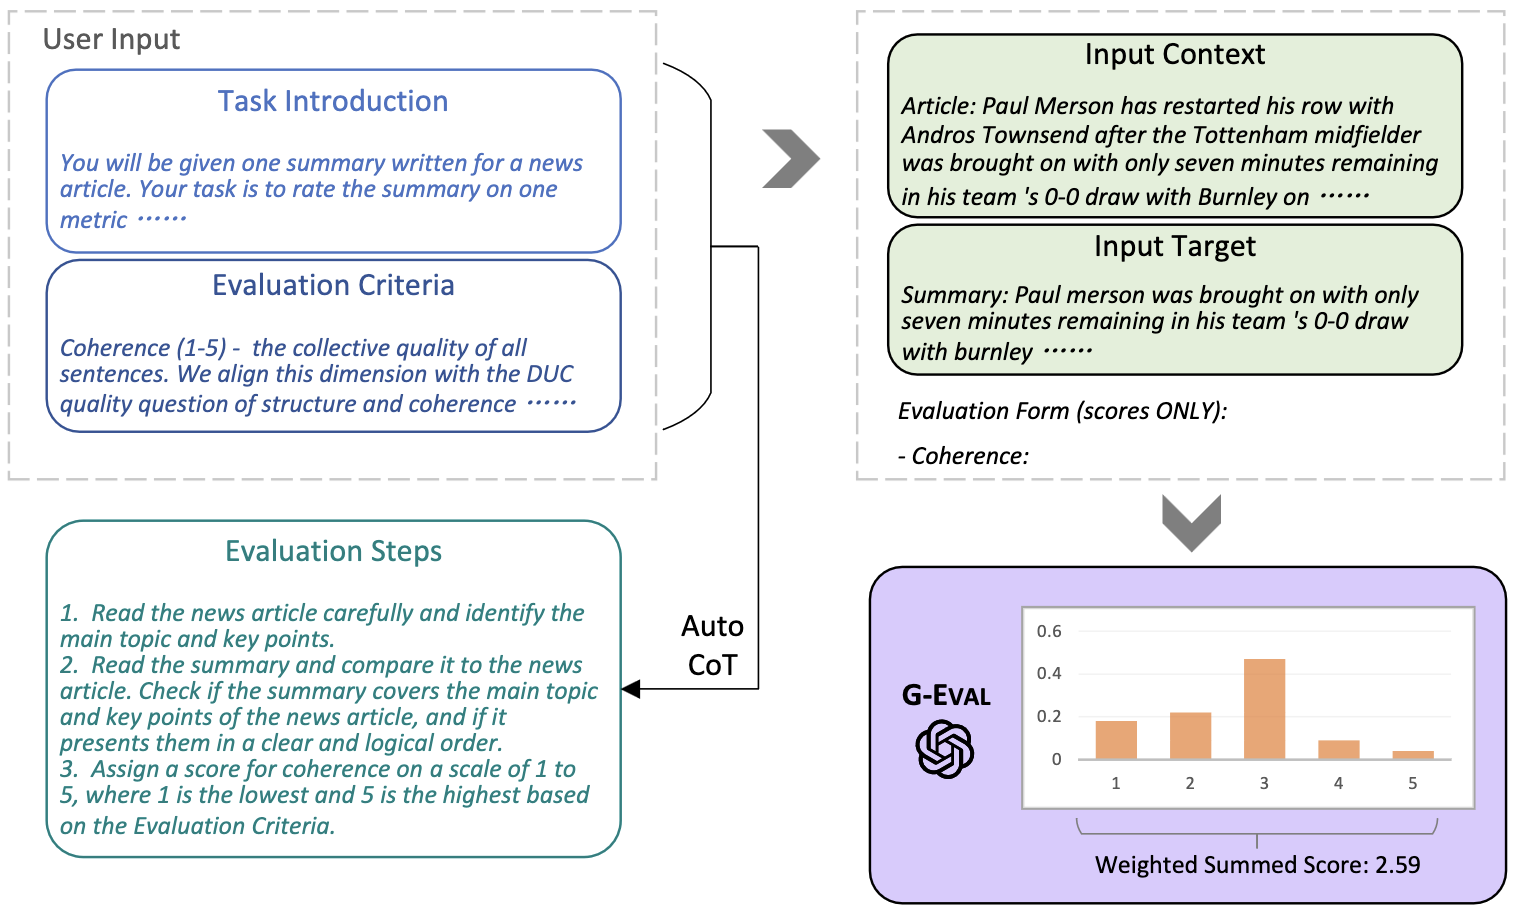
\includegraphics[width=\linewidth]{figure/geval_figure1.png}
\end{figure}
\end{column}

\begin{column}{0.39\textwidth}
The judge receives

\begin{itemize}
    \item task introduction,
    \item evaluation criteria,
    \item generated evaluation steps,
    \item the candidate output.
\end{itemize}

\end{column}

\end{columns}


Rather than use only the most likely integer score, G-Eval computes $\operatorname{score}
=
\sum_{i=1}^{n} p(s_i)\,s_i$,

where $s_i$ are allowed ratings and $p(s_i)$ their re-scaled output-token probabilities.


\end{vbframe}


% ------------------------------------------------------------------------------

\begin{vbframe}{Evaluating the Evaluator}

Standard meta-evaluation measures agreement with a
\textbf{global human ranking}.
\citebutton{Xu et al., 2025: The Progress Illusion}
{https://aclanthology.org/2025.findings-emnlp.1036/}

But can an evaluator distinguish \textbf{similarly strong systems}?

Consider only pairs with small evaluator score difference: $\left|S(\pi_1;E)-S(\pi_2;E)\right| < \Delta$

\begin{figure}
    \centering
    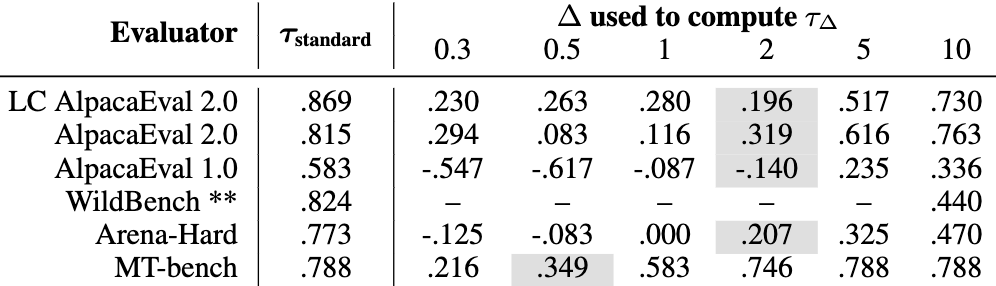
\includegraphics[width=8cm]{figure/progress_illusion_table1.png}
\end{figure}

For LC AlpacaEval 2.0:
\[
\tau = 0.869,
\qquad
\tau_{\Delta<2}=0.196.
\]

%\begin{center}
%\textbf{High global agreement can hide poor resolution for small improvements.}
%\end{center}

\end{vbframe}


% ------------------------------------------------------------------------------

\begin{vbframe}{Chatbot Arena: Human Preference at Scale}

Chatbot Arena evaluates models through anonymous pairwise comparisons. \citebutton{Chiang et al., 2024: Chatbot Arena}
{https://arxiv.org/abs/2403.04132}

\[
\text{user prompt}
\rightarrow
\begin{cases}
\text{Model A response}\\
\text{Model B response}
\end{cases}
\rightarrow
\text{human vote}.
\]

\begin{itemize}
    \item Users supply real prompts.
    \item Model identities are hidden during voting.
    \item Pairwise votes are aggregated into rankings.
\end{itemize}


\end{vbframe}


\begin{vbframe}{Chatbot Arena: Human Preference at Scale}

\begin{figure}
    \centering
    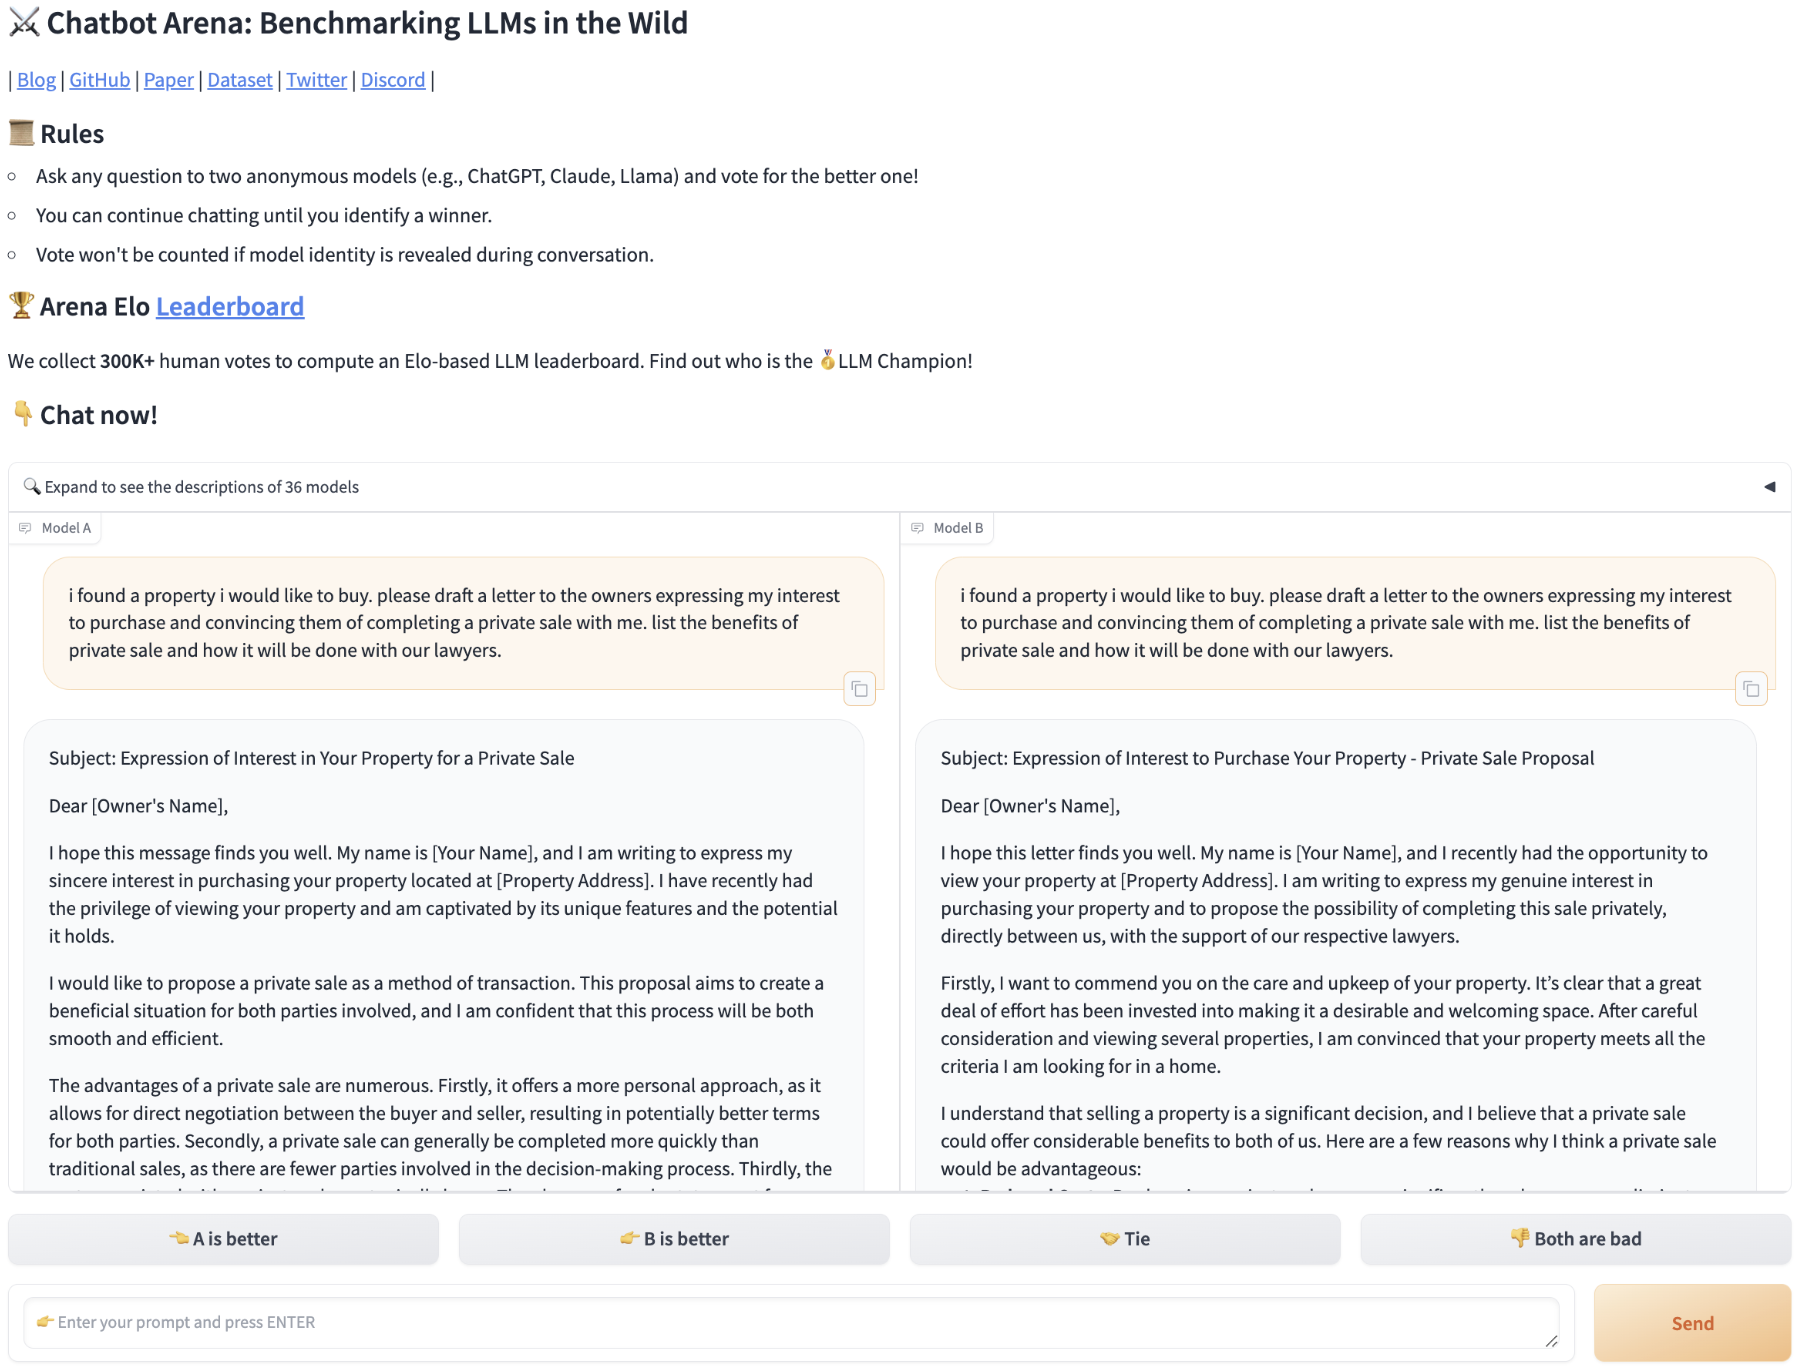
\includegraphics[width=9cm]{figure/chatbot_arena_interface.png}
\end{figure}


\end{vbframe}


% ------------------------------------------------------------------------------

\begin{vbframe}{From Votes to Rankings: Bradley--Terry}

Arena-style rankings can be modeled with Bradley--Terry scores.

For models $i$ and $j$,

\[
P(i \succ j)
=
\frac{\exp(\xi_i)}
{\exp(\xi_i)+\exp(\xi_j)}
=
\sigma(\xi_i-\xi_j).
\]

\begin{itemize}
    \item $\xi_i$: latent strength of model $i$.
    \item Only score differences matter.
    \item Pairwise human votes estimate the $\xi_i$ values.
\end{itemize}

\[
\xi_A-\xi_B=\log 3
\quad\Rightarrow\quad
P(A\succ B)=\frac{3}{4}.
\]

\citebutton{Chiang et al., 2024}
{https://arxiv.org/abs/2403.04132}

\end{vbframe}


% ------------------------------------------------------------------------------

\begin{vbframe}{Exercise: Bradley--Terry Update}

Assume model $A$ beats model $B$ and

\[
\xi_A=1.2,\qquad
\xi_B=0.4.
\]

\begin{enumerate}
    \item Compute
    \[
    p=P(A\succ B)=\sigma(\xi_A-\xi_B).
    \]

    \item For
    \[
    \mathcal{L}=-\log p,
    \]
    show that
    \[
    \frac{\partial \mathcal{L}}{\partial \xi_A}=p-1,
    \qquad
    \frac{\partial \mathcal{L}}{\partial \xi_B}=1-p.
    \]

    \item Perform one SGD step with learning rate $\eta=0.1$.
\end{enumerate}

\end{vbframe}


% ------------------------------------------------------------------------------

\begin{vbframe}{IFEval: Verifiable Instructions}

Instruction following is often open-ended.

IFEval instead uses instructions that can be checked automatically.

Examples:

\begin{itemize}
    \item write more than a given number of words,
    \item include a specified keyword,
    \item return valid JSON,
    \item avoid a particular punctuation mark,
    \item use a required number of bullet points.
\end{itemize}

\begin{figure}
    \centering
    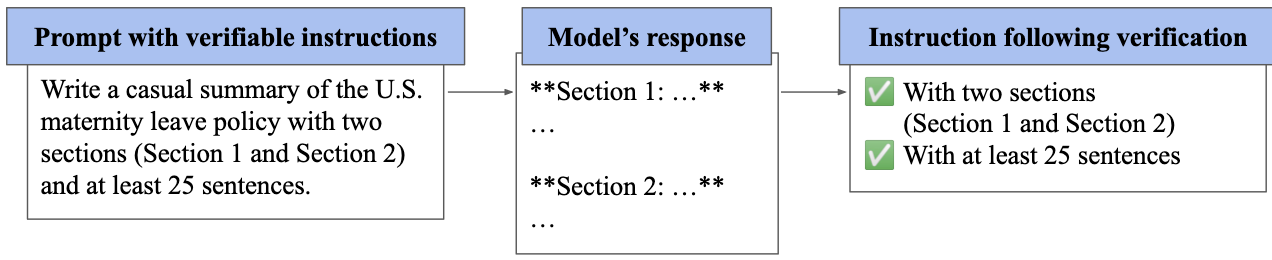
\includegraphics[width=10.5cm]{figure/ifeval_figure1.png}
\end{figure}

\citebutton{Zhou et al., 2023: IFEval}
{https://arxiv.org/abs/2311.07911}

\end{vbframe}


% ------------------------------------------------------------------------------

\begin{vbframe}{IFEval: Prompt-Level vs.\ Instruction-Level Scores}

A prompt may contain several verifiable instructions.

\begin{center}
\begin{tabular}{c|ccc}
& instruction 1 & instruction 2 & instruction 3\\
\hline
prompt 1 & 1 & 1 & 1\\
prompt 2 & 1 & 0 & 1
\end{tabular}
\end{center}

Instruction-level accuracy:

\[
\frac{5}{6}.
\]

Prompt-level accuracy:

\[
\frac{1}{2},
\]

because a prompt succeeds only if all its instructions are satisfied.

\begin{center}
\textbf{The same outputs can look better or worse depending on the level of scoring.}
\end{center}

\end{vbframe}

% ------------------------------------------------------------------------------
\begin{vbframe}{What Is Calibration?}

A model is calibrated if its confidence matches its empirical accuracy.

\[
\text{Among predictions with confidence } 0.8,
\quad
\text{about }80\%\text{ should be correct.}
\]

\begin{figure}
    \centering
    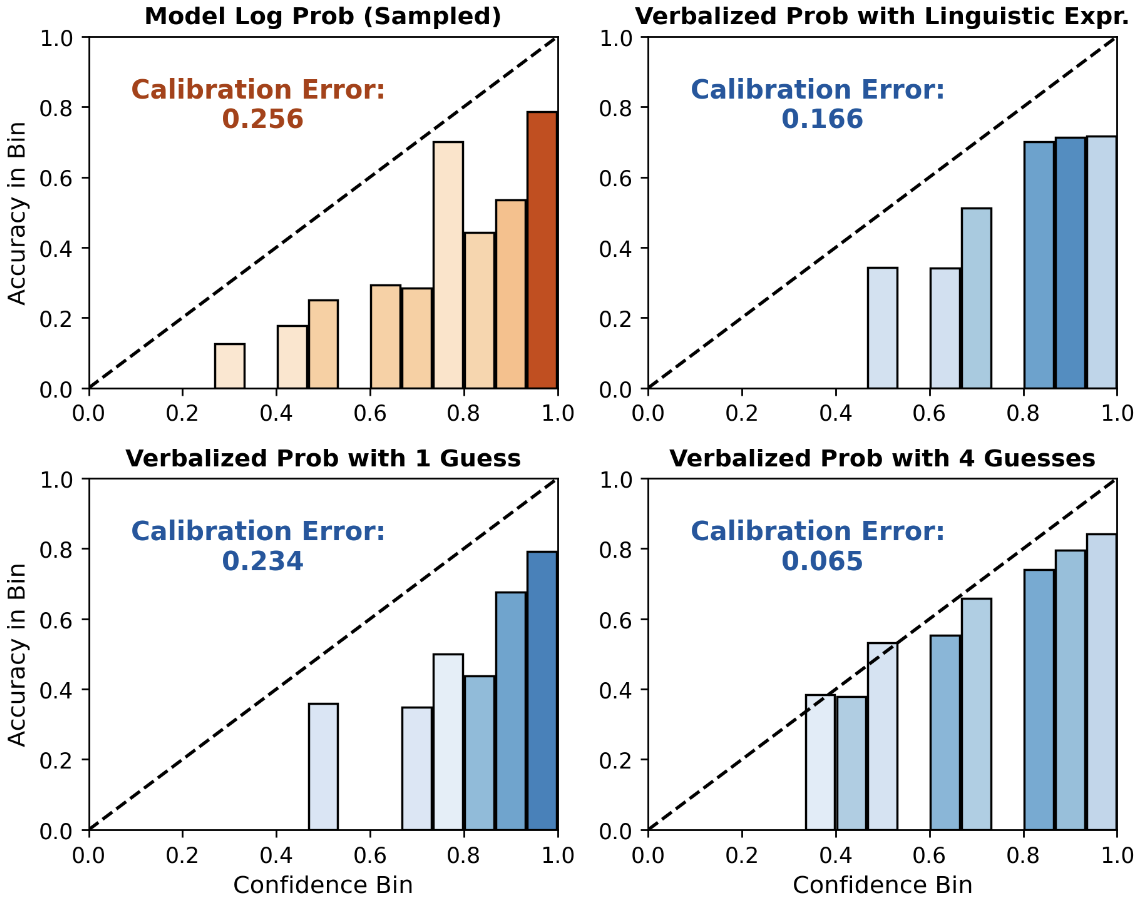
\includegraphics[width=6cm]{figure/calibration_reliability_diagram.png}
\end{figure}

\end{vbframe}


% ------------------------------------------------------------------------------

\begin{vbframe}{Where Do LLM Confidence Scores Come From?}

Several signals can be used as confidence estimates.

\begin{itemize}
    \item \textbf{Internal probability:}
          use token probabilities or answer probabilities.
    \item \textbf{Verbalized confidence:}
          ask the model to report a probability.
    \item \textbf{Self-consistency:}
          sample several answers and measure agreement.
    \item \textbf{Auxiliary estimator:}
          train a separate model to predict correctness.
    \item \textbf{Inter-model agreement:}
          compare answers from several LLMs.
\end{itemize}

\begin{center}
\textbf{Reported or estimated confidence must itself be evaluated.}
\end{center}

\citebutton{Tian et al., 2023: Just Ask for Calibration}
{https://aclanthology.org/2023.emnlp-main.330/}

\citebutton{Xia et al., 2025}
{https://aclanthology.org/2025.acl-long.188/}

\end{vbframe}


% ------------------------------------------------------------------------------

\begin{vbframe}{Calibration Metrics}

For binary correctness $y_i\in\{0,1\}$ and confidence $p_i$:

\textbf{Brier score}

\[
\operatorname{Brier}
=
\frac{1}{N}
\sum_{i=1}^{N}
(p_i-y_i)^2.
\]

\textbf{Log loss}

\[
-\frac{1}{N}
\sum_i
\left[
y_i\log p_i+
(1-y_i)\log(1-p_i)
\right].
\]

\textbf{Expected Calibration Error}

\[
\operatorname{ECE}
=
\sum_b
\frac{|S_b|}{N}
\left|
\operatorname{acc}(S_b)-\operatorname{conf}(S_b)
\right|.
\]

\end{vbframe}


% ------------------------------------------------------------------------------

\begin{vbframe}{Exercise: Brier Score}

Suppose a model answers three questions.

\[
(y_1,y_2,y_3)=(1,0,1),
\qquad
(p_1,p_2,p_3)=(0.9,0.8,0.6).
\]

\[
\operatorname{Brier}
=
\frac{
(0.9-1)^2+
(0.8-0)^2+
(0.6-1)^2
}{3}.
\]

\[
=
\frac{0.01+0.64+0.16}{3}
=
0.27.
\]

\begin{center}
\textbf{Confident mistakes are costly.}
\end{center}

\ques Compare this to always predicting confidence $0.6$.

\end{vbframe}



% ------------------------------------------------------------------------------

\begin{vbframe}{SWE-bench: Testing Code Generation}

SWE-bench contains 2,294 software-engineering tasks
from 12 popular Python repositories. \citebutton{Jimenez et al., 2023: SWE-bench}
{https://arxiv.org/abs/2310.06770}

\[
\text{issue + repository}
\rightarrow
\text{model patch}
\rightarrow
\text{tests}
\]

\begin{figure}
    \centering
    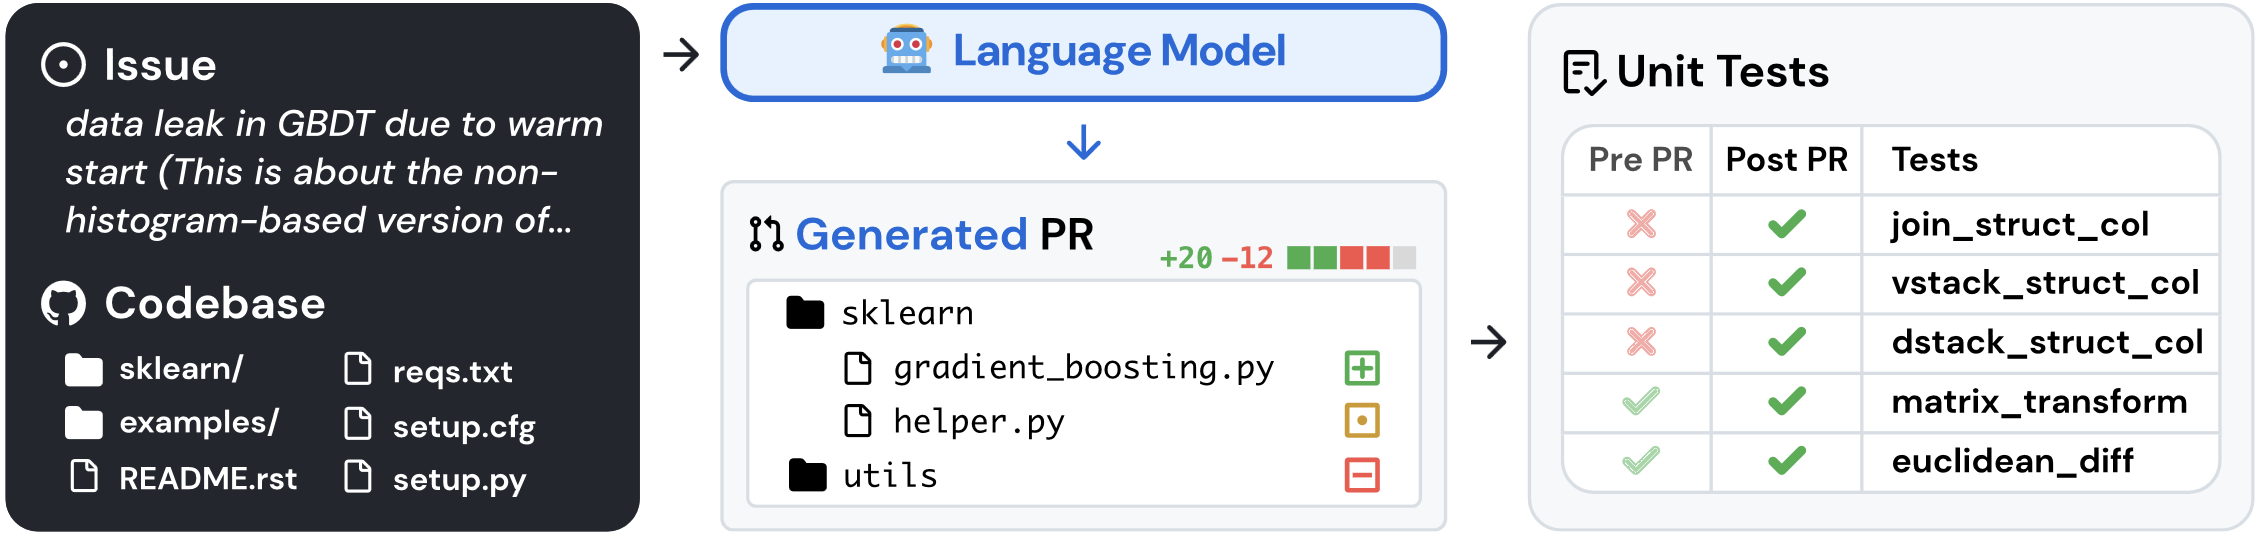
\includegraphics[width=8cm]{figure/swebench_figure1.png}
\end{figure}

A task is solved only if the generated patch fixes the issue
without breaking existing functionality. 
\textbf{Evaluation is based on executable outcomes.}

\end{vbframe}

% ------------------------------------------------------------------------------

\begin{vbframe}{OSWorld: Evaluation Through Interaction}

\begin{columns}[T,onlytextwidth]

\begin{column}{0.48\textwidth}

OSWorld evaluates agents on real computer tasks across
applications and operating systems.

\[
s_0
\rightarrow
a_1
\rightarrow
s_1
\rightarrow
\cdots
\rightarrow
s_T.
\]

The agent observes the computer state, acts through mouse and keyboard,
and is evaluated from the resulting environment state.

\begin{center}
\textbf{The target is successful task completion.}
\end{center}

\citebutton{Xie et al., 2024: OSWorld}
{https://arxiv.org/abs/2404.07972}

\end{column}

\begin{column}{0.48\textwidth}

\begin{figure}
    \centering
    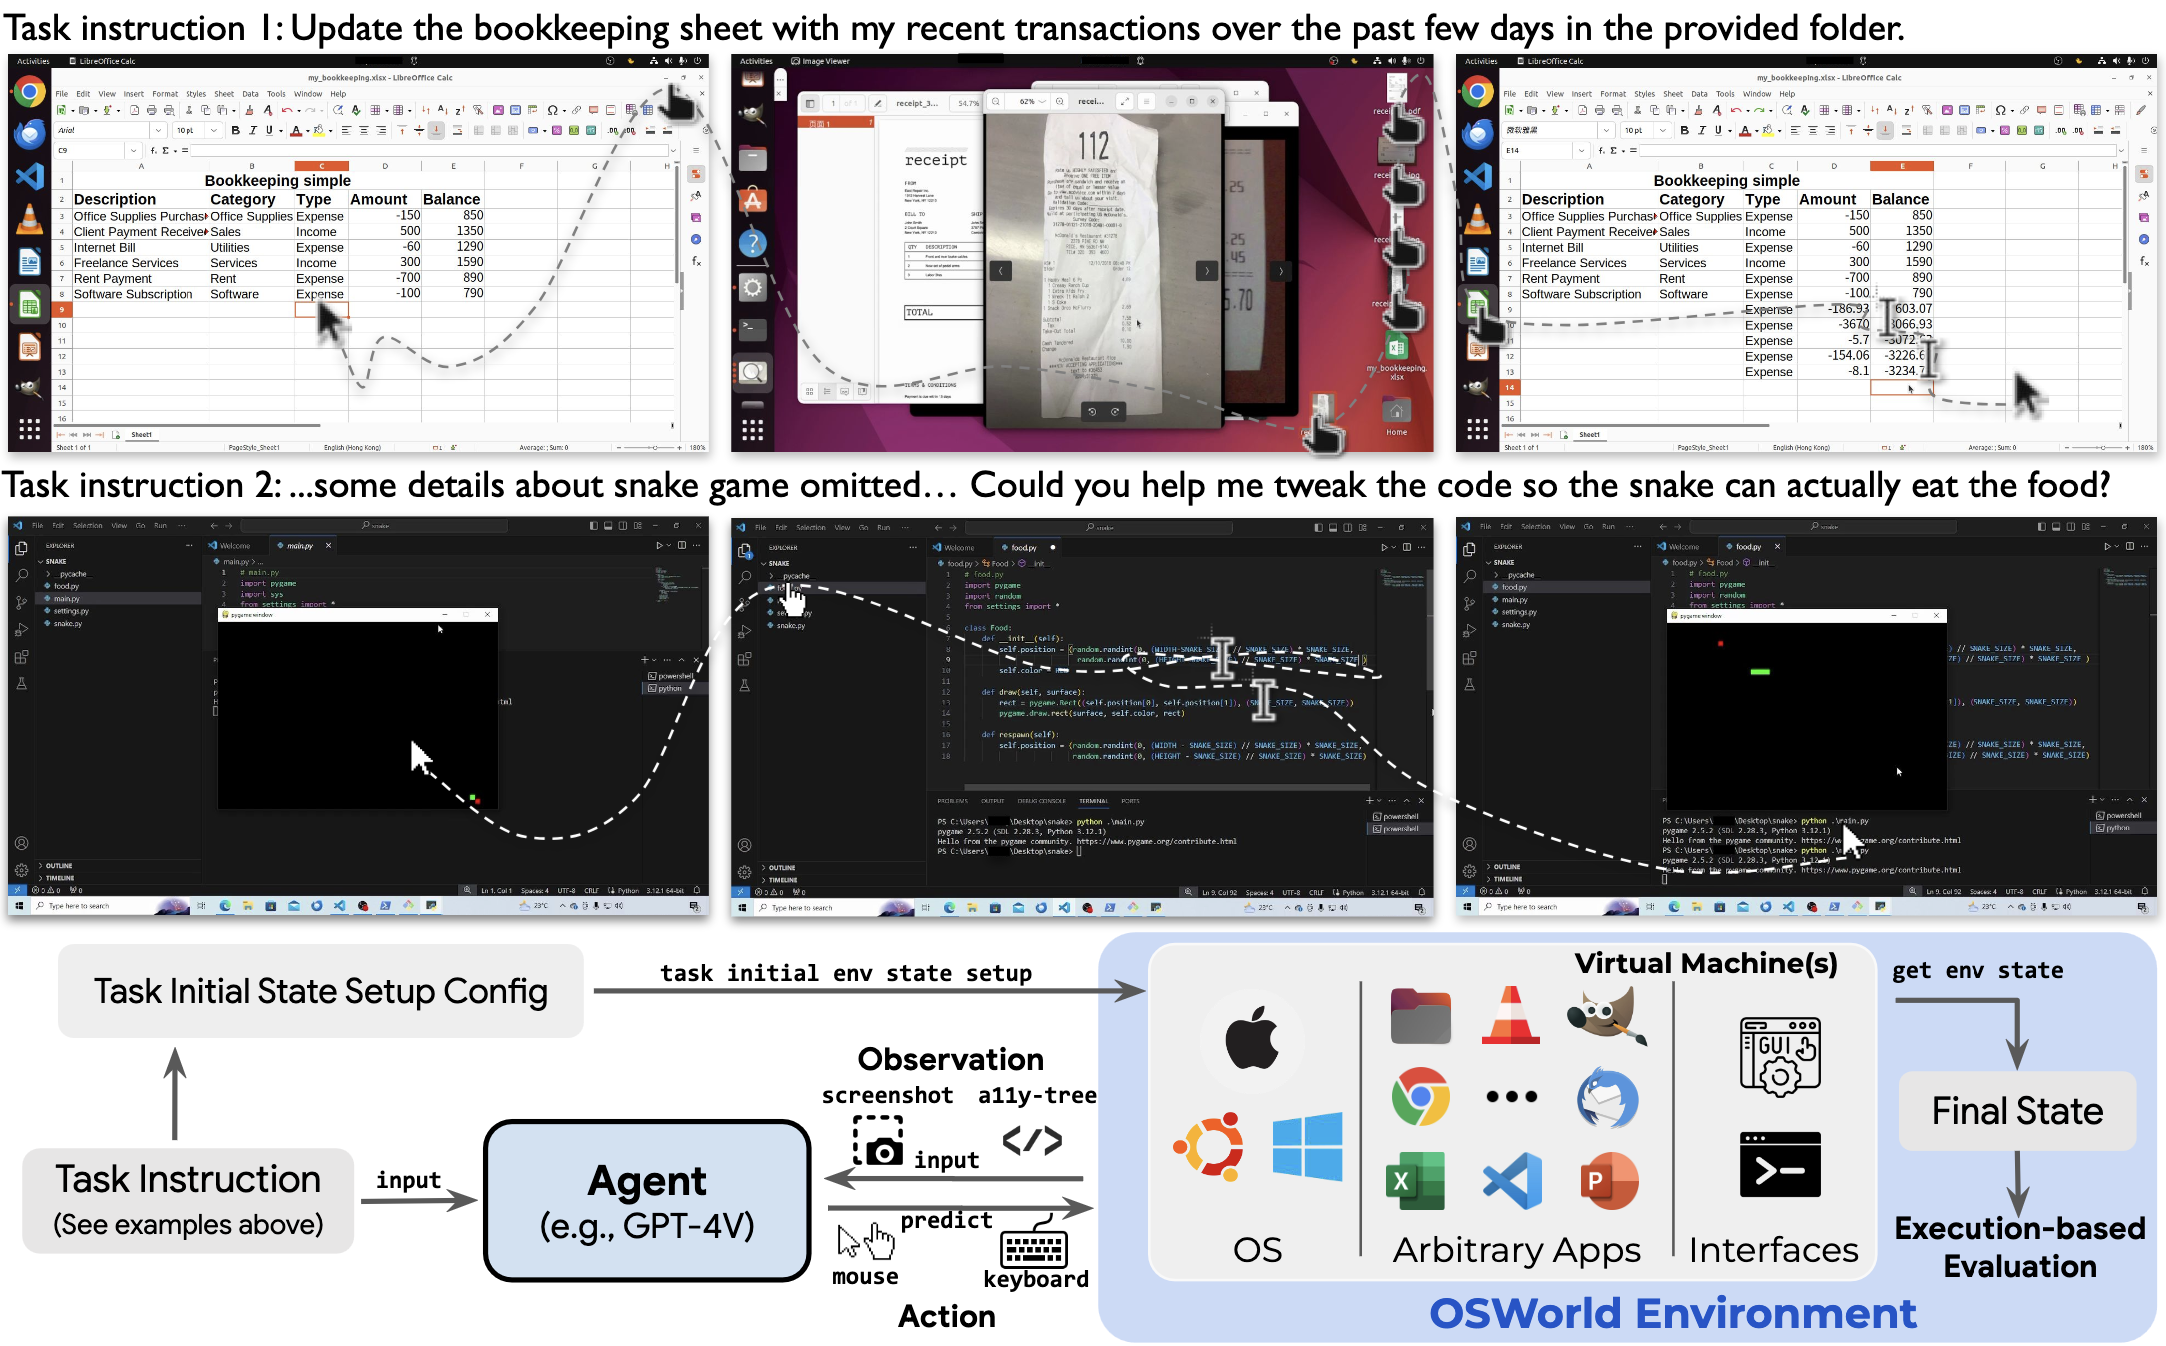
\includegraphics[width=\linewidth]{figure/osworld_figure1.png}
\end{figure}

\end{column}

\end{columns}

\end{vbframe}


% ------------------------------------------------------------------------------

\begin{frame}[plain]
\vfill
\begin{center}
{\LARGE \textbf{Benchmark Contamination}}

\medskip

{\large Has the model already seen the test set?}
\end{center}
\vfill
\end{frame}


% ------------------------------------------------------------------------------

\begin{vbframe}{What Is Benchmark Contamination?}

A benchmark should test generalization to unseen examples.

But test items may appear in training data:

\[
D_{\mathrm{train}}
\cap
D_{\mathrm{test}}
\neq
\varnothing.
\]

Contamination can include

\begin{itemize}
    \item exact duplicates,
    \item near-duplicates or paraphrases,
    \item answer options or metadata,
    \item benchmark-targeted fine-tuning.
\end{itemize}

\begin{center}
\textbf{High benchmark performance may reflect exposure,
not generalization.}
\end{center}

\end{vbframe}


% ------------------------------------------------------------------------------

\begin{vbframe}{How Can Contamination Be Detected?}
\begin{itemize}
    \item \textbf{Corpus search:}
          search known training corpora for exact or near-duplicate
          benchmark items.
    \item \textbf{Test-set slot guessing:}
          mask an answer option or unusual word and ask the model to reconstruct it.
    \item \textbf{Perturbation tests:}
          compare performance on original items with changed variants.
    \item \textbf{Clean subsets:}
          remove suspected contaminated examples and recompute performance.
\end{itemize}

\begin{figure}
    \centering
    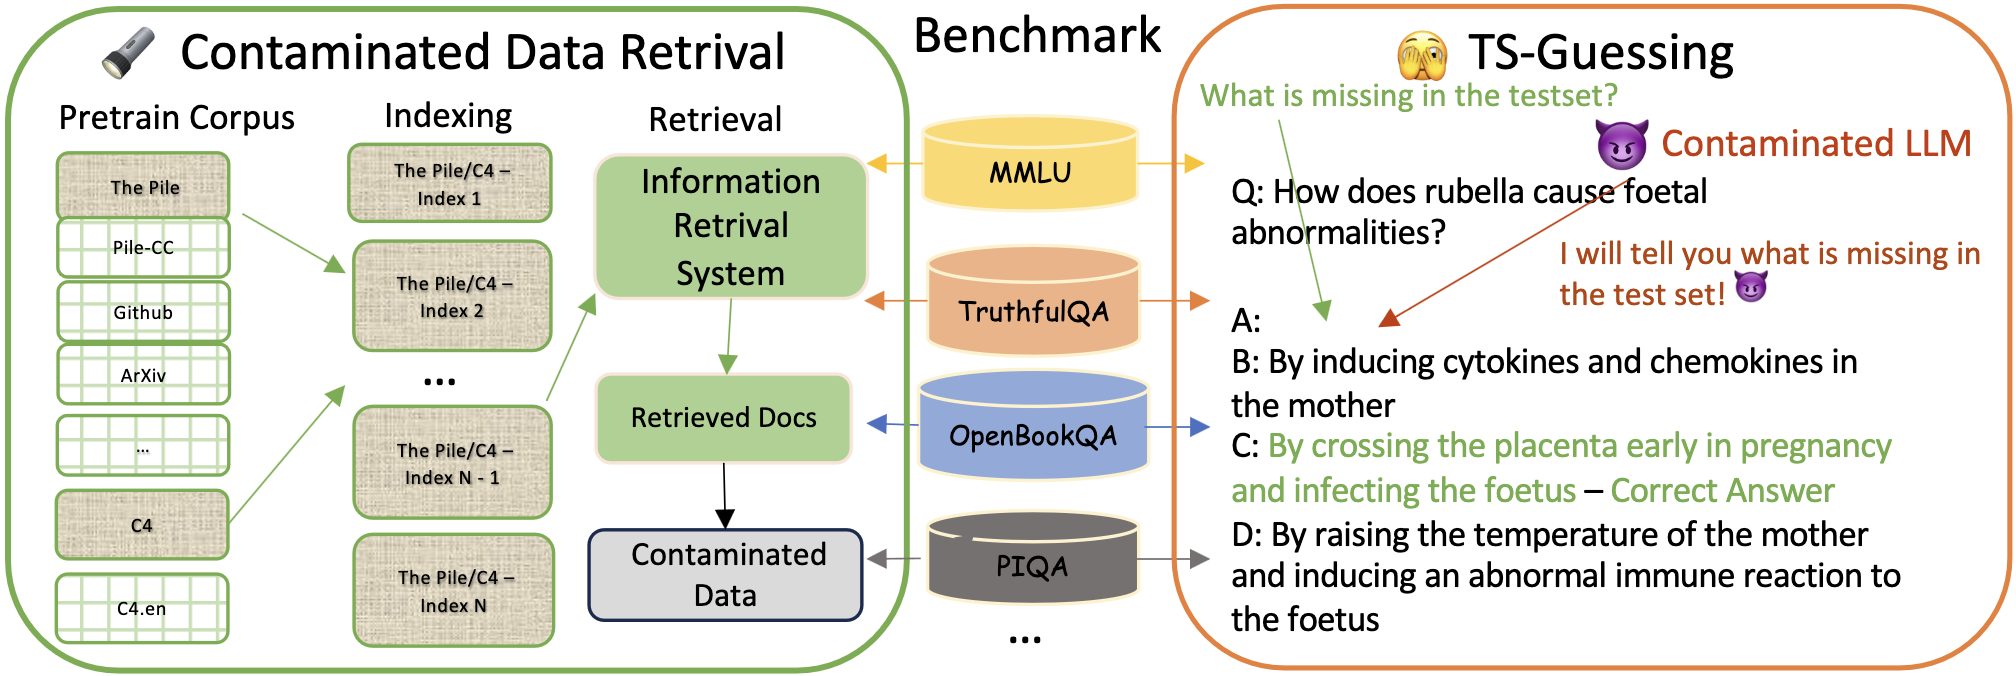
\includegraphics[width=8cm]{figure/contamination_detection.png}
\end{figure}

%\begin{center}
%\textbf{For closed models, contamination is especially hard to rule out.}
%\end{center}

\citebutton{Deng et al., 2023}
{https://arxiv.org/abs/2311.09783}

\end{vbframe}


% ------------------------------------------------------------------------------

\begin{vbframe}{Concrete Finding: Test-Set Slot Guessing}

\citebutton{Deng et al., 2023}
{https://arxiv.org/abs/2311.09783} test whether models can reconstruct hidden parts of benchmark items.

For MMLU, they hide one wrong answer option and ask the model to guess it.

\begin{itemize}
    \item ChatGPT exact-match rate: about $52\%$.
    \item GPT-4 exact-match rate: about $57\%$.
    \item Random guessing would be much lower.
\end{itemize}

\begin{figure}
    \centering
    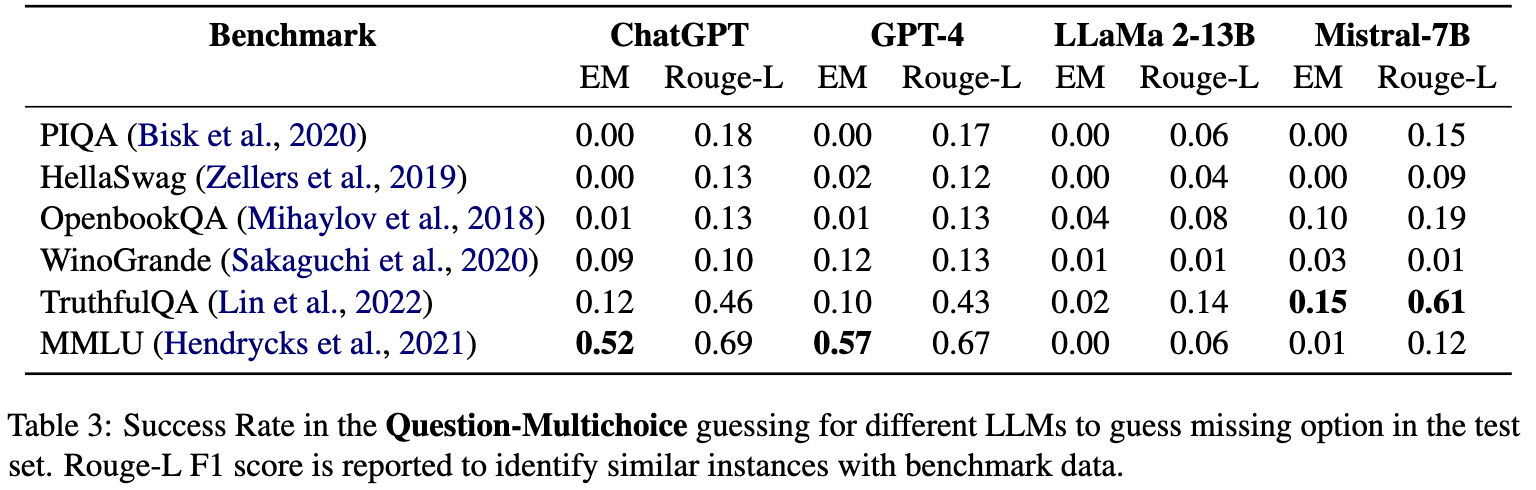
\includegraphics[width=9.5cm]{figure/ts_guessing_mmlu.png}
\end{figure}

\end{vbframe}


% ------------------------------------------------------------------------------

\begin{vbframe}{Evaluation Paradigms}

\[
\begin{array}{lll}
\textbf{MMLU}
&:&
\text{Was the selected answer correct?}
\\[0.4em]

\textbf{MT-Bench}
&:&
\text{Does a judge prefer or score the response?}
\\[0.4em]

\textbf{Chatbot Arena}
&:&
\text{Which model do humans prefer?}
\\[0.4em]

\textbf{IFEval}
&:&
\text{Were explicit instructions satisfied?}
\\[0.4em]

\textbf{Calibration}
&:&
\text{Does confidence match correctness?}
\\[0.4em]

\textbf{SWE-bench}
&:&
\text{Does the generated patch pass the tests?}
\\[0.4em]

\textbf{OSWorld}
&:&
\text{Did interaction accomplish the task?}
\\[0.4em]
\textbf{Contamination tests}
&:&
\text{Was the benchmark truly unseen?}
\end{array}
\]

\end{vbframe}


% ------------------------------------------------------------------------------

\begin{vbframe}{LLM Evaluation: Main Takeaways}

\begin{itemize}

    \item \textbf{Judgment for Open-ended outputs:}
    MT-Bench uses LLM judges; Arena uses human pairwise preferences.

    \item \textbf{IFEval} checks explicit instruction constraints automatically.

    \item Accuracy can be complemented by \textbf{confidence calibration metrics}.

    \item \textbf{SWE-bench} and \textbf{OSWorld} measure execution and interaction outcomes.

    \item \textbf{Contamination}
     can make test performance invalid.

\end{itemize}

\end{vbframe}

\endlecture
\end{document}
